%\documentclass[11pt, draft]{article}
\documentclass[11pt]{article}
\usepackage{lindrew}
\usepackage{xcolor}
\usepackage{amsmath}
\usepackage{amssymb}
\usepackage{tikz}
\usepackage{hyperref}
\usepackage{fontspec}
\title{Physics 2301: Intermediate Mechanics II}
\author{Lecturer: \textbf{Professor Antonio Boveia}\\Notes by: Farhan Sadeek}
\date{Spring 2025}

\begin{document}

\maketitle

%%%%%%%%%%%%%%%%%%%%%%%%%%%%
\section{January 7, 2025}
\subsection{Course Introduction}

Dr.\ Boveia talked about the course and we will head towards relativistic mechanics. In this course, we will master the concepts from Physics 1250 but more broadly. \textbf{Tuesday} is the lecture day and \textbf{Wednesday,} Thursday, and Friday are the problem-solving days. The grading scale would be on the \textbf{Standard Ohio State} grading scale. There might be a curve but it will only curve up, not down. Our grade would rely on \textbf{Quizzes (20\%), Midterm (20\%), Final (20\%), Homework (30\%)}, and \textbf{Participation (10\%)}. The exams are \textbf{open-book, open-notes, and open-internet}.

\subsection{Success Tips}
Here are some tips to succeed in Physics 2301:
\begin{itemize}
    \item \textbf{Attend all lectures and problem-solving sessions:} Regular attendance will help you understand the material better and keep up with the course pace.
    \item \textbf{Stay organized:} Keep track of all assignments, quizzes, and exam dates. Use a planner or digital calendar to manage your time effectively.
    \item \textbf{Participate actively:} Engage in class discussions and ask questions whenever you have doubts. Participation counts towards your grade.
    \item \textbf{Form study groups:} Collaborate with your peers to discuss concepts and solve problems. Group study can provide different perspectives and enhance understanding.
    \item \textbf{Utilize office hours:} Take advantage of Dr.\ Boveia's office hours to seek clarification on topics you find challenging.
    \item \textbf{Practice regularly:} Consistently work on homework and additional problems to reinforce your understanding of relativistic mechanics.
    \item \textbf{Review notes:} Regularly review your lecture notes and summarize key points to aid retention.
    \item \textbf{Use available resources:} Make use of the textbook, online resources, and any supplementary materials provided by Dr.\ Boveia.
    \item \textbf{Stay healthy:} Ensure you get enough rest, eat well, and manage stress to maintain your overall well-being.
\end{itemize}

\subsection{Review of Vectors and Matrices}
\begin{definition}
    A \textbf{scalar quantity} is a quantity with only magnitude. Examples include mass, temperature, and time.
\end{definition}

\begin{definition}
    A \textbf{vector quantity} is a quantity with both magnitude and direction. Examples include displacement, velocity, and force. Vectors follow a different set of rules compared to scalars. For example, there are two multiplication rules for vectors: \textbf{Dot Product} and \textbf{Cross Product}. The dot product results in a scalar quantity while the cross product results in a vector quantity.

    \[
        |\vec{v}| = \text{Length and} \quad \vec{v} = \frac{|\vec{v}|}{\sqrt{3}}(V_x, V_y, V_z) \text{ if } \vec{v} = \langle V_x, V_y, V_z \rangle
    \]

    Scalar \(\times\) Vector = Vector \\
    Vector \(\cdot\) Vector = Scalar (Dot Product or Inner Product) \\
    \[
        \vec{v} \cdot \vec{v} = V_x \cdot V_x + V_y \cdot V_y + V_z \cdot V_z = |\vec{v}|^2
    \]
    \[
        \vec{A} \cdot \vec{B} = A_x \cdot B_x + A_y \cdot B_y + A_z \cdot B_z = |\vec{A}| |\vec{B}| \cos \theta
    \]
    \[
        \vec{A} = A_x \hat{x} + A_y \hat{y} + A_z \hat{z}
    \]
    \(\hat{x}\) = `Unit Vector' \(|\hat{x}| = 1\)
    \[
        \vec{A} \cdot \vec{B} = (A_x \hat{x} + A_y \hat{y} + A_z \hat{z}) \cdot (B_x \hat{x} + B_y \hat{y} + B_z \hat{z}) = A_x B_x + A_y B_y + A_z B_z
    \]

    \(\hat{x}, \hat{y}, \hat{z}\) form an orthogonal normal basis, meaning that \(\hat{x} \cdot \hat{y} = 0\)
    \[
        \hat{x} \cdot \hat{y} = 0, \quad \hat{y} \cdot \hat{z} = 0, \quad \hat{z} \cdot \hat{x} = 0
    \]
    Here, Ortho means that \(\hat{x} \cdot \hat{y} = 0\) and Normal means that \(\hat{x} \cdot \hat{x} = 1\)
\end{definition}

Vector \(\times\) Vector = Cross Product = Vector
\[
    \vec{A} \times \vec{B} = |\vec{A}| |\vec{B}| \sin \theta \hat{n}
\]

\[
    \vec{A} \times \vec{B} = \begin{vmatrix}
        \hat{x} & \hat{y} & \hat{z} \\
        A_x     & A_y     & A_z     \\
        B_x     & B_y     & B_z
    \end{vmatrix}
\]

\begin{figure}[h]
    \centering
    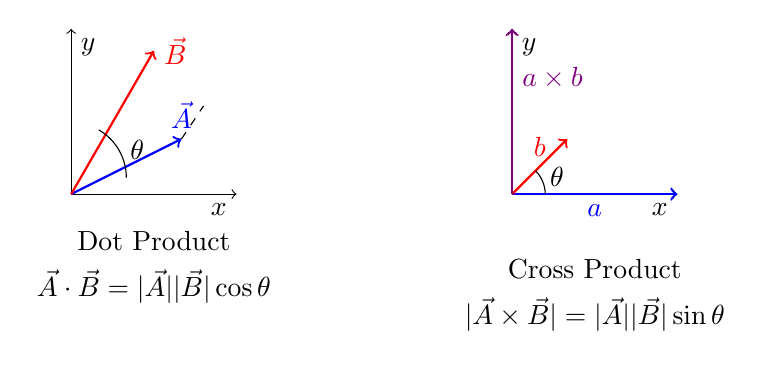
\begin{tikzpicture}[scale=0.7]
        % Axes for dot product
            \begin{scope}[xshift=-4cm]
                \draw[->] (0,0) -- (3,0) node[anchor=north east]{$x$};
                \draw[->] (0,0) -- (0,3) node[anchor=north west]{$y$};
                \draw[->, thick, blue] (0,0) -- (2,1) node[anchor=south]{$\vec{A}$};
                \draw[->, thick, red] (0,0) -- (1.5,2.6) node[anchor=west]{$\vec{B}$};
                \draw[dashed] (2,1) -- (2.4,1.6);
                \draw (1.0,0.3) arc (0:60:1);
                \node at (1.2,0.8) {$\theta$};
                \node[below] at (1.5,-0.5) {Dot Product};
                \node[below] at (1.5,-1.2) {$\vec{A}\cdot\vec{B} = |\vec{A}||\vec{B}|\cos\theta$};
            \end{scope}

            % Axes for cross product
            \begin{scope}[xshift=4cm]
                \draw[->] (0,0,0) -- (3,0,0) node[anchor=north east]{$x$};
                \draw[->] (0,0,0) -- (0,3,0) node[anchor=north west]{$y$};
                \draw[->, thick, blue] (0,0) -- (3,0) node[midway,below]{$a$};
                \draw[->, thick, red] (0,0) -- (1,1) node[midway,above]{$b$};
                \draw[->, thick, blue!50!red] (0,0) -- (0,3) node[pos=0.7,right]{$a\times b$};
                \draw (0.6,0) arc [start angle=0,end angle=45,radius=0.6] node[pos=0.7,right]{$\theta$};
                \node[below] at (1.5,-1) {Cross Product};
                \node[below] at (1.5,-1.7) {$|\vec{A}\times\vec{B}| = |\vec{A}||\vec{B}|\sin\theta$};
            \end{scope}
    \end{tikzpicture}
    \caption{Geometric interpretation of dot and cross products}
\end{figure}

\textbf{Dot product} is just the magnitude of the projection of \(\vec{A}\) onto \(\vec{B}\).

\[
    \vec{A} \times \vec{B} = |\vec{A}| |\vec{B}| \sin \theta \hat{n}
\]

Dot product is the component of $\vec{B}$ along $\vec{A}$. The dot product is a scalar quantity.

The cross product is a vector that is perpendicular to both \(\vec{A}\) and \(\vec{B}\) (\(\vec{A} \perp \vec{B}\)). The magnitude of the cross product is the area of the parallelogram formed by \(\vec{A}\) and \(\vec{B}\). The direction of the cross product follows the right-hand rule.

\[
    \vec{A} \times \vec{B} = \begin{vmatrix}
        \hat{x} & \hat{y} & \hat{z} \\
        A_x     & A_y     & A_z     \\
        B_x     & B_y     & B_z
    \end{vmatrix}
\]

\subsection{Matrices}
A \textbf{matrix} is a rectangular array of numbers arranged in rows and columns. Matrices are used to represent linear transformations and solve systems of linear equations.

\begin{definition}
    A matrix \(A\) with \(m\) rows and \(n\) columns is denoted as \(A \in \mathbb{R}^{m \times n}\). Each element of the matrix is denoted as \(a_{ij}\), where \(i\) is the row index and \(j\) is the column index.
\end{definition}

\begin{equation}
    A = \begin{pmatrix}
        a_{11} & a_{12} & \cdots & a_{1n} \\
        a_{21} & a_{22} & \cdots & a_{2n} \\
        \vdots & \vdots & \ddots & \vdots \\
        a_{m1} & a_{m2} & \cdots & a_{mn}
    \end{pmatrix}
\end{equation}

\textbf{Matrix Addition:} Two matrices \(A\) and \(B\) of the same dimension can be added by adding their corresponding elements.
\begin{equation}
    (A + B)_{ij} = a_{ij} + b_{ij}
\end{equation}

\textbf{Matrix Multiplication:} The product of two matrices \(A \in \mathbb{R}^{m \times n}\) and \(B \in \mathbb{R}^{n \times p}\) is a matrix \(C \in \mathbb{R}^{m \times p}\) where each element is given by the dot product of the corresponding row of \(A\) and column of \(B\).
\begin{equation}
    c_{ij} = \sum_{k=1}^{n} a_{ik} b_{kj}
\end{equation}

\textbf{Identity Matrix:} The identity matrix \(I\) is a square matrix with ones on the diagonal and zeros elsewhere. It acts as the multiplicative identity for matrices.
\begin{equation}
    I = \begin{pmatrix}
        1 & 0 & \cdots & 0 \\
        0 & 1 & \cdots & 0 \\
        \vdots & \vdots & \ddots & \vdots \\
        0 & 0 & \cdots & 1
    \end{pmatrix}
\end{equation}

\textbf{Transpose of a Matrix:} The transpose of a matrix \(A\), denoted \(A^T\), is obtained by swapping its rows and columns.
\begin{equation}
    (A^T)_{ij} = a_{ji}
\end{equation}

\textbf{Determinant of a Matrix:} The determinant is a scalar value that can be computed from the elements of a square matrix and encodes certain properties of the matrix. For a \(2 \times 2\) matrix, the determinant is given by:
\begin{equation}
    \det(A) = \begin{vmatrix}
        a & b \\
        c & d
    \end{vmatrix} = ad - bc
\end{equation}

\textbf{Inverse of a Matrix:} The inverse of a square matrix \(A\), denoted \(A^{-1}\), is the matrix such that \(AA^{-1} = A^{-1}A = I\). A matrix is invertible if and only if its determinant is non-zero.
\begin{equation}
    A^{-1} = \frac{1}{\det(A)} \text{adj}(A)
\end{equation}
where \(\text{adj}(A)\) is the adjugate of \(A\).

\begin{figure}[h]
    \centering
    \begin{tikzpicture}
        \matrix[matrix of math nodes,left delimiter={(},right delimiter={)}] (m) {
            a_{11} & a_{12} & \cdots & a_{1n} \\
            a_{21} & a_{22} & \cdots & a_{2n} \\
            \vdots & \vdots & \ddots & \vdots \\
            a_{m1} & a_{m2} & \cdots & a_{mn} \\
        };
    \end{tikzpicture}
    \caption{Example of a matrix}
\end{figure}

\section{January 8, 2025}

%\section{January 10, 2025}
%\section{January 13, 2025}
%\section{January 15, 2025}
%\section{January 17, 2025}
%\section{January 20, 2025}
%\section{January 22, 2025}
%\section{January 24, 2025}
%\section{January 27, 2025}
%\section{January 29, 2025}
%\section{January 31, 2025}
%\section{February 3, 2025}
%\section{February 5, 2025}
%\section{February 7, 2025}
%\section{February 10, 2025}
%\section{February 12, 2025}
%\section{February 14, 2025}
%\section{February 17, 2025}
%\section{February 19, 2025}
%\section{February 21, 2025}
%\section{February 24, 2025}
%\section{February 26, 2025}
%\section{February 28, 2025}
%\section{March 3, 2025}
%\section{March 5, 2025}
%\section{March 7, 2025}
%\section{March 17, 2025}
%\section{March 19, 2025}
%\section{March 21, 2025}
%\section{March 24, 2025}
%\section{March 26, 2025}
%\section{March 28, 2025}
%\section{March 31, 2025}
%\section{April 2, 2025}
%\section{April 4, 2025}
%\section{April 7, 2025}
%\section{April 9, 2025}
%\section{April 11, 2025}
%\section{April 14, 2025}
%\section{April 16, 2025}
%\section{April 18, 2025}
%\section{April 21, 2025}
%\section{April 23, 2025}
%\section{April 25, 2025}
%\section{April 28, 2025}

\end{document}
